% VerdeAI gap-analysis pipeline — research report / thesis figure.
%
% Standalone: compiles on its own (Overleaf, or `pdflatex`) to one
% cropped PDF you can \includegraphics{} directly, or convert to PNG:
%   pdflatex verdeai-report-figure.tex
%   pdftoppm -png -r 300 verdeai-report-figure.pdf verdeai-report-figure
%
% To embed inside an existing report/thesis instead of standalone:
%   1. Copy \begin{tikzpicture} ... \end{tikzpicture} into your own
%        \begin{figure}[t] \centering ... \caption{...} \label{...} \end{figure}
%   2. Copy the \usetikzlibrary line and \definecolor/\tikzset blocks
%      into your preamble.
%
% Three rows (not one long row) to keep the figure narrow enough for a
% single column: row 1 is document ingestion (7 boxes), rows 2-3 are
% the per-clause loop (5 boxes each), so the widest row is 7 boxes —
% about the same width as the ingestion row alone.
\documentclass[tikz, border=6mm]{standalone}
\usetikzlibrary{shapes.geometric, arrows.meta, positioning, calc}

% ---- palette: muted, print-safe. One hue per shape category, so the
% legend maps onto shape vocabulary and the figure still reads in
% grayscale (shape carries meaning; color is a secondary cue). ----
\definecolor{inkcolor}{HTML}{17241B}
\definecolor{mutedtext}{HTML}{4D5D4F}
\definecolor{terminalfill}{HTML}{F2F3EF}
\definecolor{iofill}{HTML}{B7C6DA}
\definecolor{decisionfill}{HTML}{E6D3A3}
\definecolor{processfill}{HTML}{BFD3BC}
\definecolor{aifill}{HTML}{CBB9D6}
\definecolor{reportfill}{HTML}{3E5C43}
\definecolor{abstainfill}{HTML}{D9CBB8}

\begin{document}
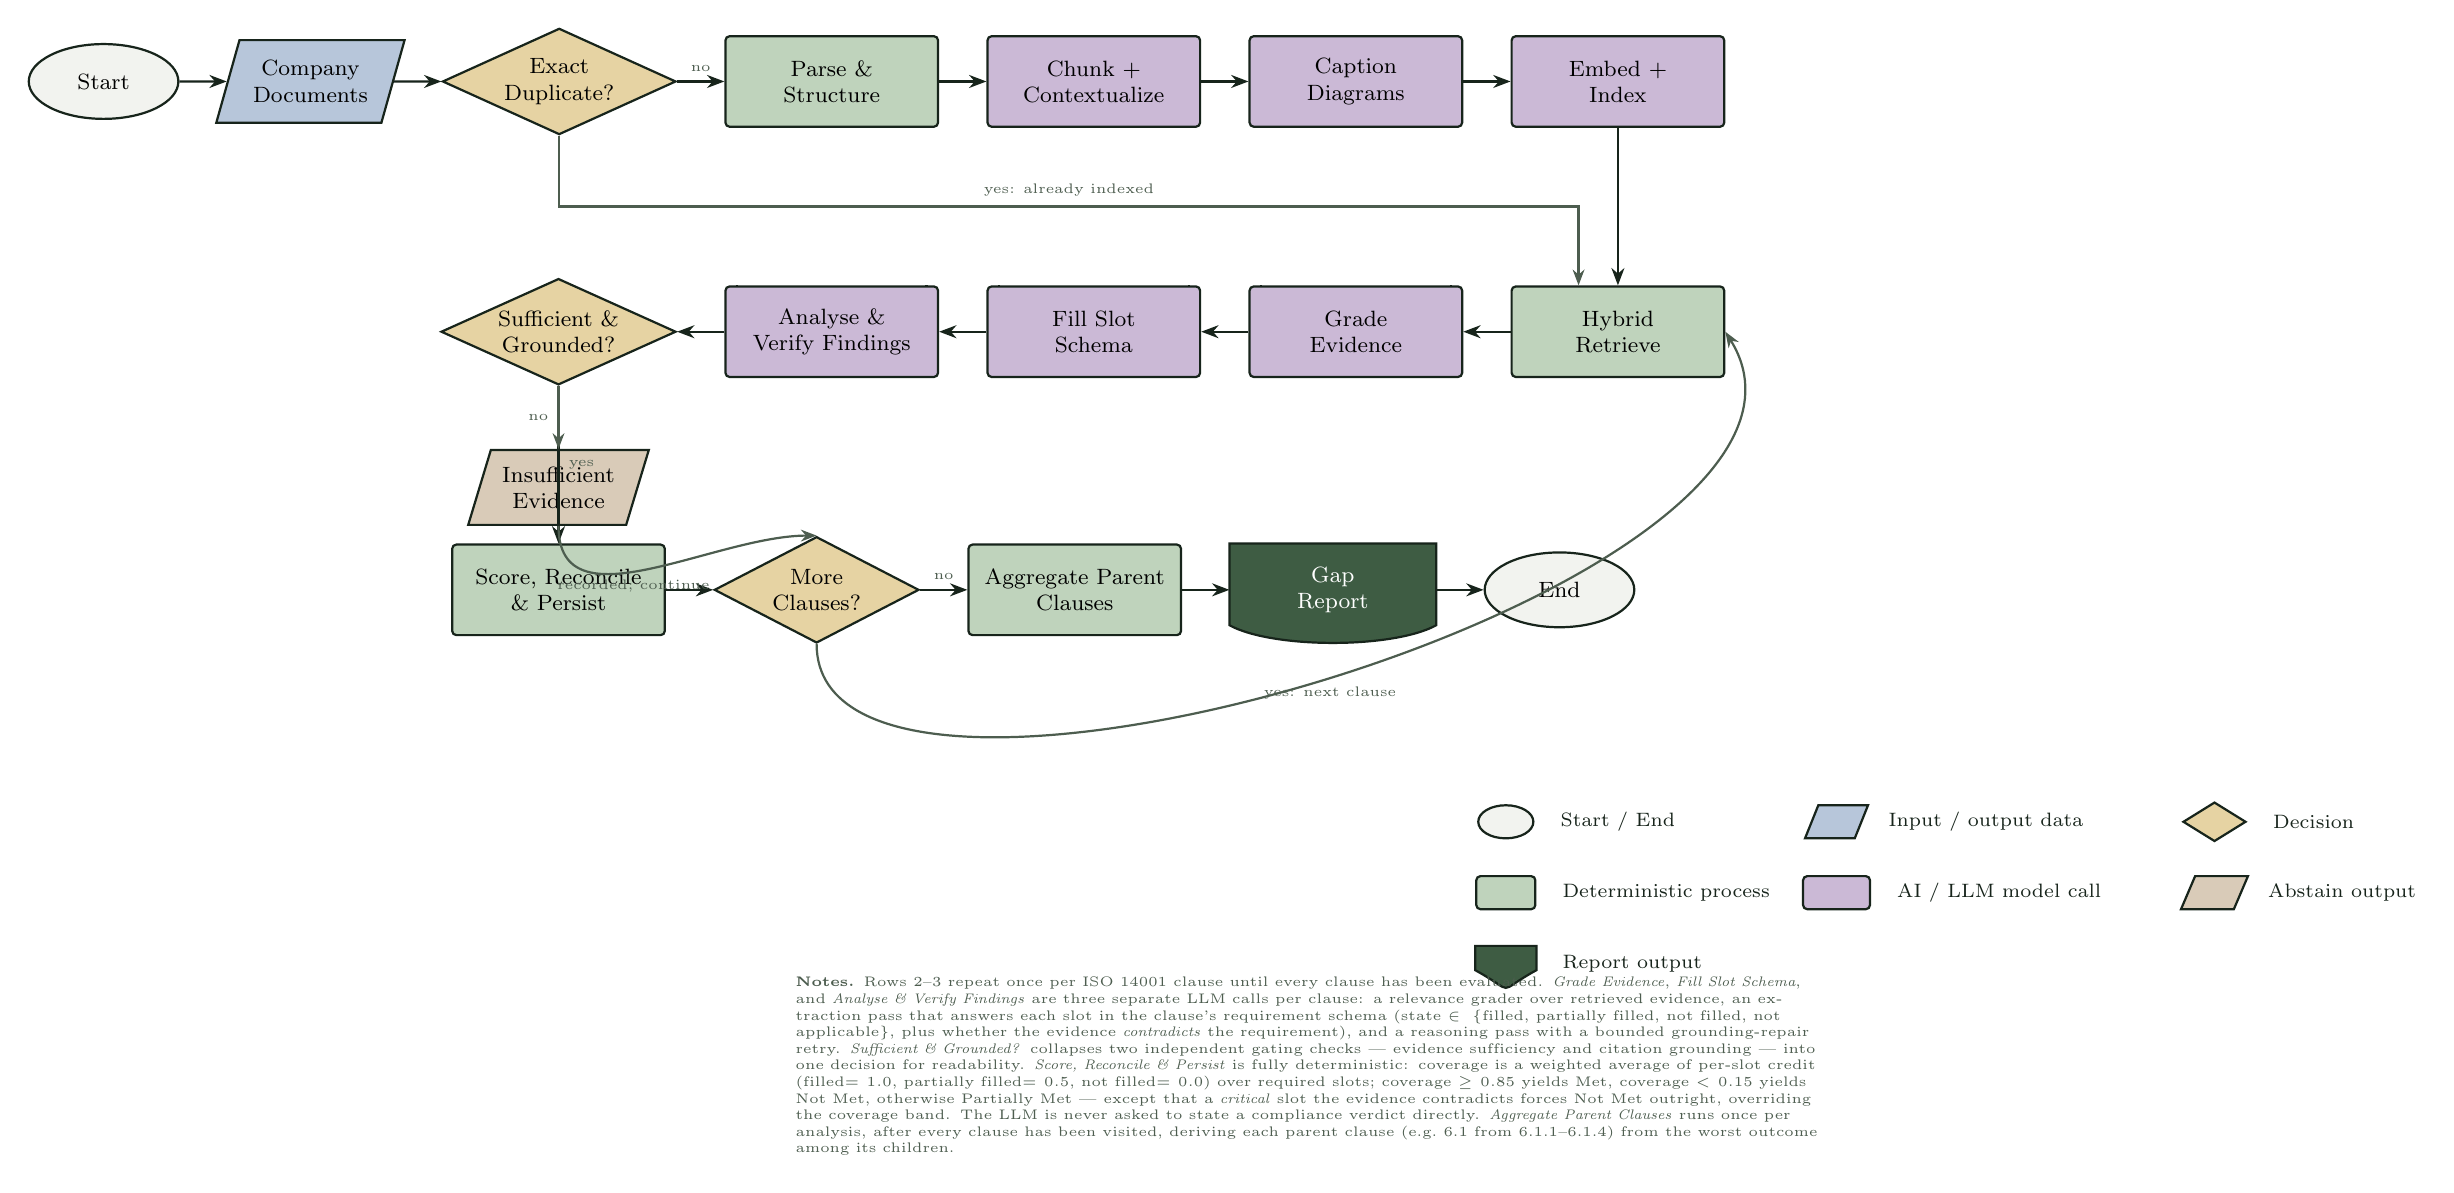
\begin{tikzpicture}[
  >=Stealth,
  every node/.style={font=\footnotesize},
  node distance=6mm and 6mm,
  align=center,
  thick,
]

% ---------------------------------------------------------------
% Node style vocabulary — one style per flowchart meaning.
% ---------------------------------------------------------------
\tikzset{
  terminal/.style={
    ellipse, draw=inkcolor, fill=terminalfill,
    minimum width=1.9cm, minimum height=0.95cm,
  },
  io/.style={
    trapezium, trapezium left angle=70, trapezium right angle=110,
    trapezium stretches=true,
    draw=inkcolor, fill=iofill,
    minimum width=2.4cm, minimum height=1.05cm,
  },
  abstain/.style={
    trapezium, trapezium left angle=70, trapezium right angle=110,
    trapezium stretches=true,
    draw=inkcolor, fill=abstainfill,
    minimum width=2.3cm, minimum height=0.95cm,
  },
  decision/.style={
    diamond, draw=inkcolor, fill=decisionfill, aspect=2.3,
    inner sep=1pt, minimum width=2.6cm, minimum height=1.35cm,
  },
  process/.style={
    rectangle, rounded corners=1.5pt, draw=inkcolor, fill=processfill,
    minimum width=2.7cm, minimum height=1.15cm,
  },
  subprocess/.style={
    rectangle, rounded corners=1.5pt, draw=inkcolor, fill=aifill,
    minimum width=2.7cm, minimum height=1.15cm,
    append after command={
      \pgfextra{
        \draw[inkcolor]
          ($(\tikzlastnode.north west)!0.16cm!(\tikzlastnode.north east)$)
          -- ($(\tikzlastnode.south west)!0.16cm!(\tikzlastnode.south east)$);
        \draw[inkcolor]
          ($(\tikzlastnode.north east)!0.16cm!(\tikzlastnode.north west)$)
          -- ($(\tikzlastnode.south east)!0.16cm!(\tikzlastnode.south west)$);
      }
    },
  },
  flowline/.style={-{Stealth[length=2.2mm]}, inkcolor},
  branchline/.style={-{Stealth[length=2mm]}, mutedtext},
}

% Hand-built "document" symbol (rectangle, wavy bottom edge) drawn at
% the position/size of an existing invisible node #1, labelled #2.
\newcommand{\documentshape}[2]{
  \draw[inkcolor, fill=reportfill]
    (#1.north west) -- (#1.north east)
    -- ($(#1.south east)+(0,0.14)$)
    .. controls ($(#1.south east)+(-0.55,-0.16)$) and ($(#1.south west)+(0.55,-0.16)$) ..
    ($(#1.south west)+(0,0.14)$) -- cycle;
  \node[text=white, align=center] at (#1) {#2};
}

% =================================================================
% ROW 1 — document ingestion & indexing (services/document-processor,
% stages 1-6: dedup, parse, chunk+contextualize, caption, embed, index).
% Left to right.
% =================================================================
\node[terminal]                              (start)    {Start};
\node[io,         right=of start]            (docs)     {Company\\Documents};
\node[decision,   right=of docs]             (dup)      {Exact\\Duplicate?};
\node[process,    right=of dup]              (parse)    {Parse \&\\Structure};
\node[subprocess, right=of parse]            (chunk)    {Chunk +\\Contextualize};
\node[subprocess, right=of chunk]            (caption)  {Caption\\Diagrams};
\node[subprocess, right=of caption]          (embed)    {Embed +\\Index};

% =================================================================
% ROW 2 — evidence retrieval & grading, per ISO 14001 clause. Right to
% left, directly below row 1, entering under "Embed + Index".
% =================================================================
\node[process,    below=20mm of embed]       (retrieve) {Hybrid\\Retrieve};
\node[subprocess, left=of retrieve]          (grade)    {Grade\\Evidence};
\node[subprocess, left=of grade]             (fill)     {Fill Slot\\Schema};
\node[subprocess, left=of fill]              (analyse)  {Analyse \&\\Verify Findings};
\node[decision,   left=of analyse]           (ok)       {Sufficient \&\\Grounded?};

\node[abstain, below=8mm of ok]              (insuff)   {Insufficient\\Evidence};

% =================================================================
% ROW 3 — deterministic decision, loop control, wrap-up. Left to
% right, directly below row 2, entering under "Sufficient & Grounded?".
% =================================================================
\node[process,    below=20mm of ok]          (score)    {Score, Reconcile\\\& Persist};
\node[decision,   right=of score]            (more)     {More\\Clauses?};
\node[process,    right=of more]             (aggregate){Aggregate Parent\\Clauses};
\node[rectangle, minimum width=2.6cm, minimum height=1.15cm,
      right=of aggregate]                    (reportbox){};
\node[terminal,   right=of reportbox]        (end)      {End};

% =================================================================
% Main flow — row 1
% =================================================================
\draw[flowline] (start) -- (docs);
\draw[flowline] (docs) -- (dup);
\draw[flowline] (dup) -- node[above, font=\tiny, text=mutedtext]{no} (parse);
\draw[flowline] (parse) -- (chunk);
\draw[flowline] (chunk) -- (caption);
\draw[flowline] (caption) -- (embed);

% bend: row 1 -> row 2, first pass over a clause
\draw[flowline] (embed.south) -- (retrieve.north);

% Main flow — row 2 (right to left)
\draw[flowline] (retrieve) -- (grade);
\draw[flowline] (grade) -- (fill);
\draw[flowline] (fill) -- (analyse);
\draw[flowline] (analyse) -- (ok);

% bend: row 2 -> row 3
\draw[flowline] (ok.south) -- node[right, font=\tiny, text=mutedtext]{yes} (score.north);

% Main flow — row 3 (left to right)
\draw[flowline] (score) -- (more);
\draw[flowline] (more) -- node[above, font=\tiny, text=mutedtext]{no} (aggregate);
\draw[flowline] (aggregate) -- (reportbox);
\draw[flowline] (reportbox) -- (end);

% =================================================================
% Branch 1 — duplicate short-circuit: the document's chunks are
% already indexed from a prior upload, so skip straight to retrieval.
% =================================================================
\coordinate (bypassLane)  at ($(dup.south)+(0,-0.9)$);
\coordinate (bypassEntry) at ($(retrieve.north)+(-0.5,0)$);
\coordinate (bypassTurn)  at (bypassEntry |- bypassLane);
\draw[branchline]
  (dup.south) -- (bypassLane)
  -- node[above, font=\tiny, text=mutedtext]{yes: already indexed} (bypassTurn)
  -- (bypassEntry);

% =================================================================
% Branch 2 — evidence insufficient, or the verdict could not be
% grounded within the retry budget: abstain, a short drop into the
% genuinely clear gap between rows 2 and 3.
% =================================================================
\draw[branchline] (ok.south) -- node[left, font=\tiny, text=mutedtext]{no} (insuff.north);

% Insufficient Evidence still counts as this clause's persisted
% result, so it re-joins the loop exactly like a scored verdict does.
% Drawn as a short local arc (not a routed rectilinear path) so it
% stays correct regardless of the exact node geometry.
\draw[branchline] (insuff.south) .. controls +(0,-1.3) and +(-1.3,0) ..
  node[below, font=\tiny, text=mutedtext, xshift=-2mm]{recorded; continue} (more.north);

% =================================================================
% Branch 3 — loop back for the next ISO 14001 clause. Drawn as a wide
% arc from "More Clauses?" back up to "Hybrid Retrieve", swinging
% below and around row 3 rather than a precise rectilinear route —
% robust to the exact width of row 3, which may change if boxes are
% relabelled.
% =================================================================
\draw[branchline] (more.south) .. controls +(0,-3.2) and +(2.0,-3.2) ..
  node[below, font=\tiny, text=mutedtext]{yes: next clause} (retrieve.east);

\documentshape{reportbox}{Gap\\Report}

% =================================================================
% Legend
% =================================================================
\begin{scope}[shift={($(end.south west)+(0,-2.6)$)}]
  \node[terminal, minimum width=0.7cm, minimum height=0.42cm, font=\tiny] (l1) at (0,0) {};
  \node[right=2mm of l1, font=\scriptsize, text=inkcolor] {Start / End};

  \node[io, minimum width=0.8cm, minimum height=0.42cm, font=\tiny] (l2) at (4.2,0) {};
  \node[right=2mm of l2, font=\scriptsize, text=inkcolor] {Input / output data};

  \node[decision, minimum width=0.8cm, minimum height=0.5cm, font=\tiny] (l3) at (9.0,0) {};
  \node[right=2mm of l3, font=\scriptsize, text=inkcolor] {Decision};

  \node[process, minimum width=0.75cm, minimum height=0.42cm, font=\tiny] (l4) at (0,-0.9) {};
  \node[right=2mm of l4, font=\scriptsize, text=inkcolor] {Deterministic process};

  \node[subprocess, minimum width=0.85cm, minimum height=0.42cm, font=\tiny] (l5) at (4.2,-0.9) {};
  \node[right=2mm of l5, font=\scriptsize, text=inkcolor] {AI / LLM model call};

  \node[abstain, minimum width=0.85cm, minimum height=0.42cm, font=\tiny] (l6) at (9.0,-0.9) {};
  \node[right=2mm of l6, font=\scriptsize, text=inkcolor] {Abstain output};

  \node[rectangle, minimum width=0.75cm, minimum height=0.42cm] (l7) at (0,-1.8) {};
  \documentshape{l7}{}
  \node[right=2mm of l7, font=\scriptsize, text=inkcolor] {Report output};
\end{scope}

% =================================================================
% Caption note — the deliberate simplifications this figure makes,
% stated explicitly so the diagram cannot be misread as the literal
% node graph.
% =================================================================
\node[font=\tiny, text=mutedtext, below=6mm of end, xshift=-3.2cm, yshift=-3.7cm,
      text width=13cm, align=left]
  {\textbf{Notes.} Rows 2--3 repeat once per ISO~14001 clause until every clause has been
  evaluated. \emph{Grade Evidence}, \emph{Fill Slot Schema}, and \emph{Analyse \& Verify
  Findings} are three separate LLM calls per clause: a relevance grader over retrieved
  evidence, an extraction pass that answers each slot in the clause's requirement schema
  (state $\in\{$filled, partially filled, not filled, not applicable$\}$, plus whether the
  evidence \emph{contradicts} the requirement), and a reasoning pass with a bounded
  grounding-repair retry. \emph{Sufficient \& Grounded?} collapses two independent gating
  checks --- evidence sufficiency and citation grounding --- into one decision for
  readability. \emph{Score, Reconcile \& Persist} is fully deterministic: coverage is a
  weighted average of per-slot credit (filled$=1.0$, partially filled$=0.5$, not
  filled$=0.0$) over required slots; coverage~$\geq 0.85$ yields Met, coverage~$<0.15$
  yields Not Met, otherwise Partially Met --- except that a \emph{critical} slot the
  evidence contradicts forces Not Met outright, overriding the coverage band. The LLM is
  never asked to state a compliance verdict directly. \emph{Aggregate Parent Clauses} runs
  once per analysis, after every clause has been visited, deriving each parent clause
  (e.g.\ 6.1 from 6.1.1--6.1.4) from the worst outcome among its children.};

\end{tikzpicture}
\end{document}
